
\appendix
\onecolumn
% Insert your Lean Canvas and other appendices.
\section{Scrum}
\label{appendix:appendix1}
Scrum methodology was adopted in this project. Team held weekly or biweekly scrum meeting were everybody presented his work and talked about future task. As for a software stack team was using:

\begin{itemize}
    \item Slack for communication.
    \item Slack extensions for GitHub ant trello for notifications.
    \item Github for source control.
    \item Trello for sprint tasks management.
    \item Zoom for meetings.
    \item Azure DevOps for CI/CD.
    \item Notion, google suit for project wiki.
\end{itemize}


% --------------------
\section{Code}
\label{appendix:appendix2}
\subsection{Class diagram}
\label{appendix:classDiagram}
\begin{figure}[H]
    \centering
    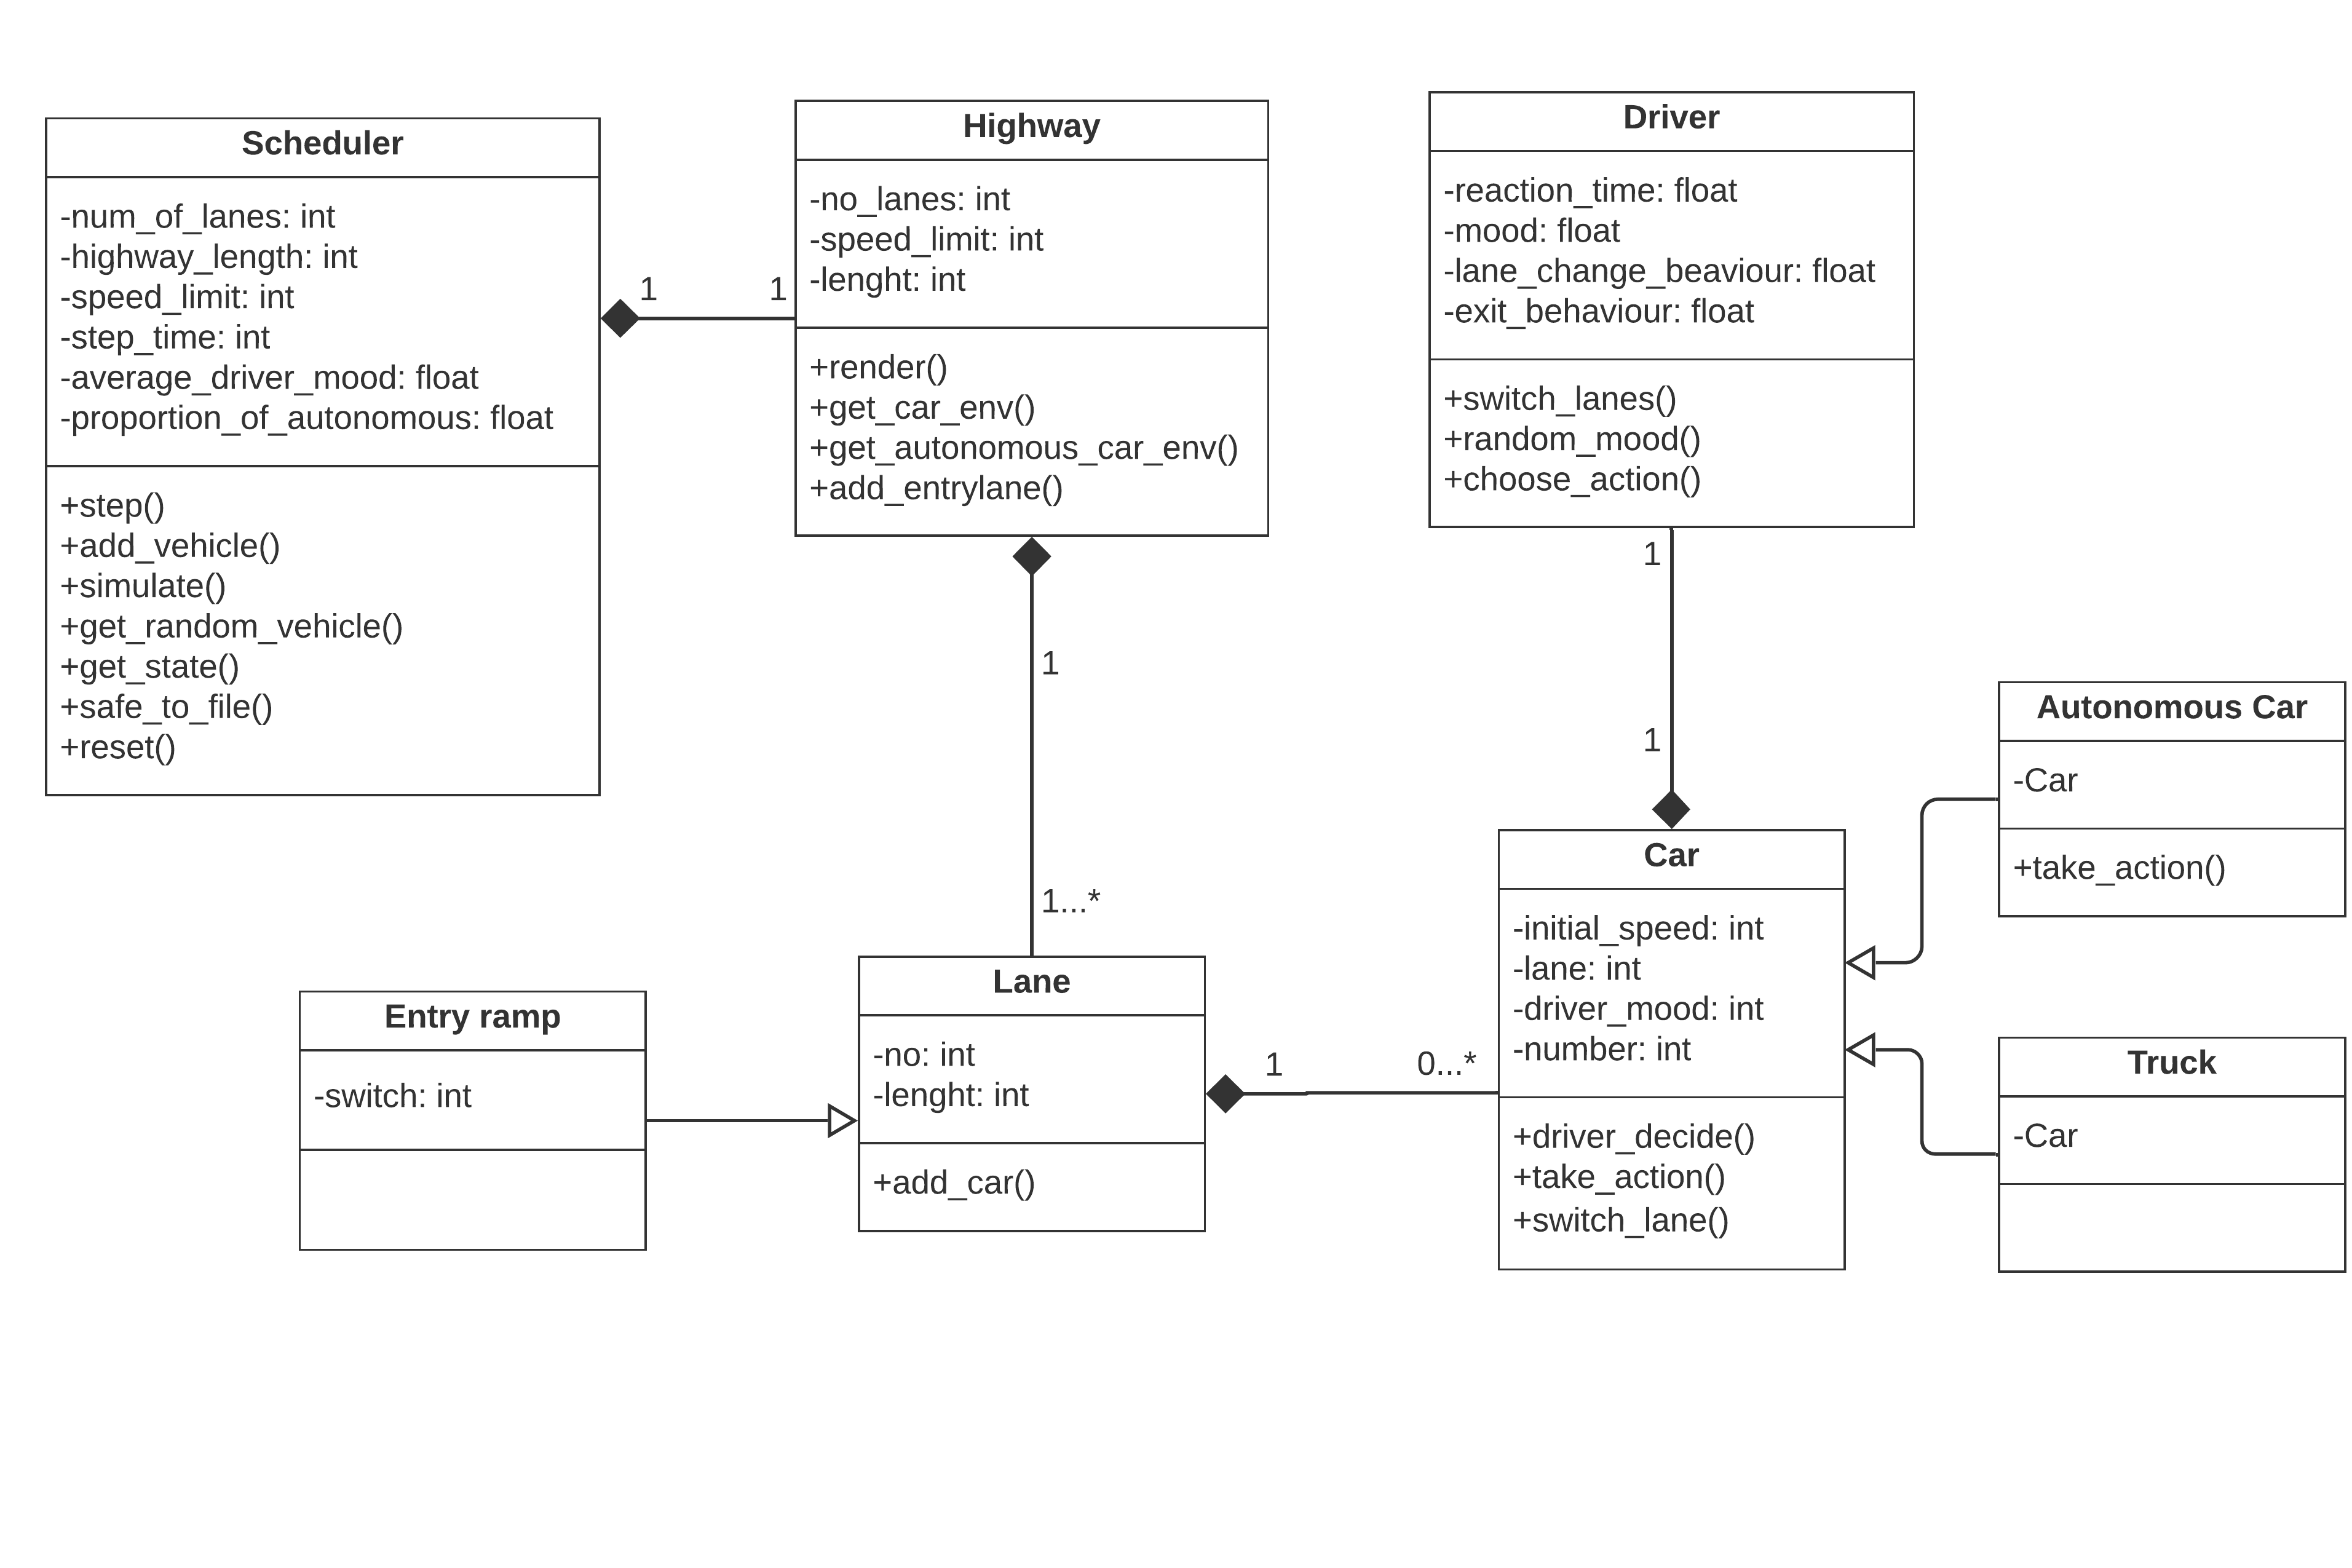
\includegraphics[width=\linewidth]{images/UML class (1).png}
    \caption{Class Diagram}
    \label{fig:classDiagram}
\end{figure}


\subsection{Testing}
Automatized testing was introduced using Azure DevOps pipelines. For every push and PR in the repository, it was tested if simulation is able to produce any result as well if there is an option to save and restore data from simulation.

\begin{figure}[H]
    \centering
    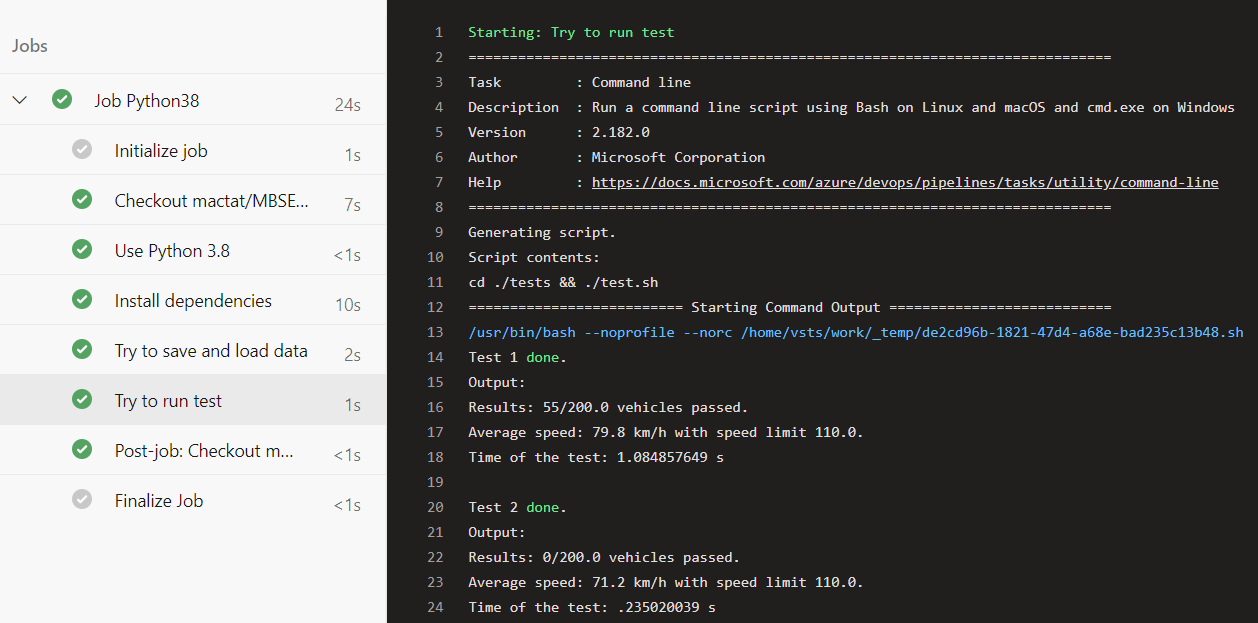
\includegraphics[width=0.8\linewidth]{images/automatic-test.png}
    \caption{Automated testing approach}
    \label{fig:automated-testing}
\end{figure}

\subsection{Output}
\label{appendix:color-output}
\begin{figure}[H]
    \centering
    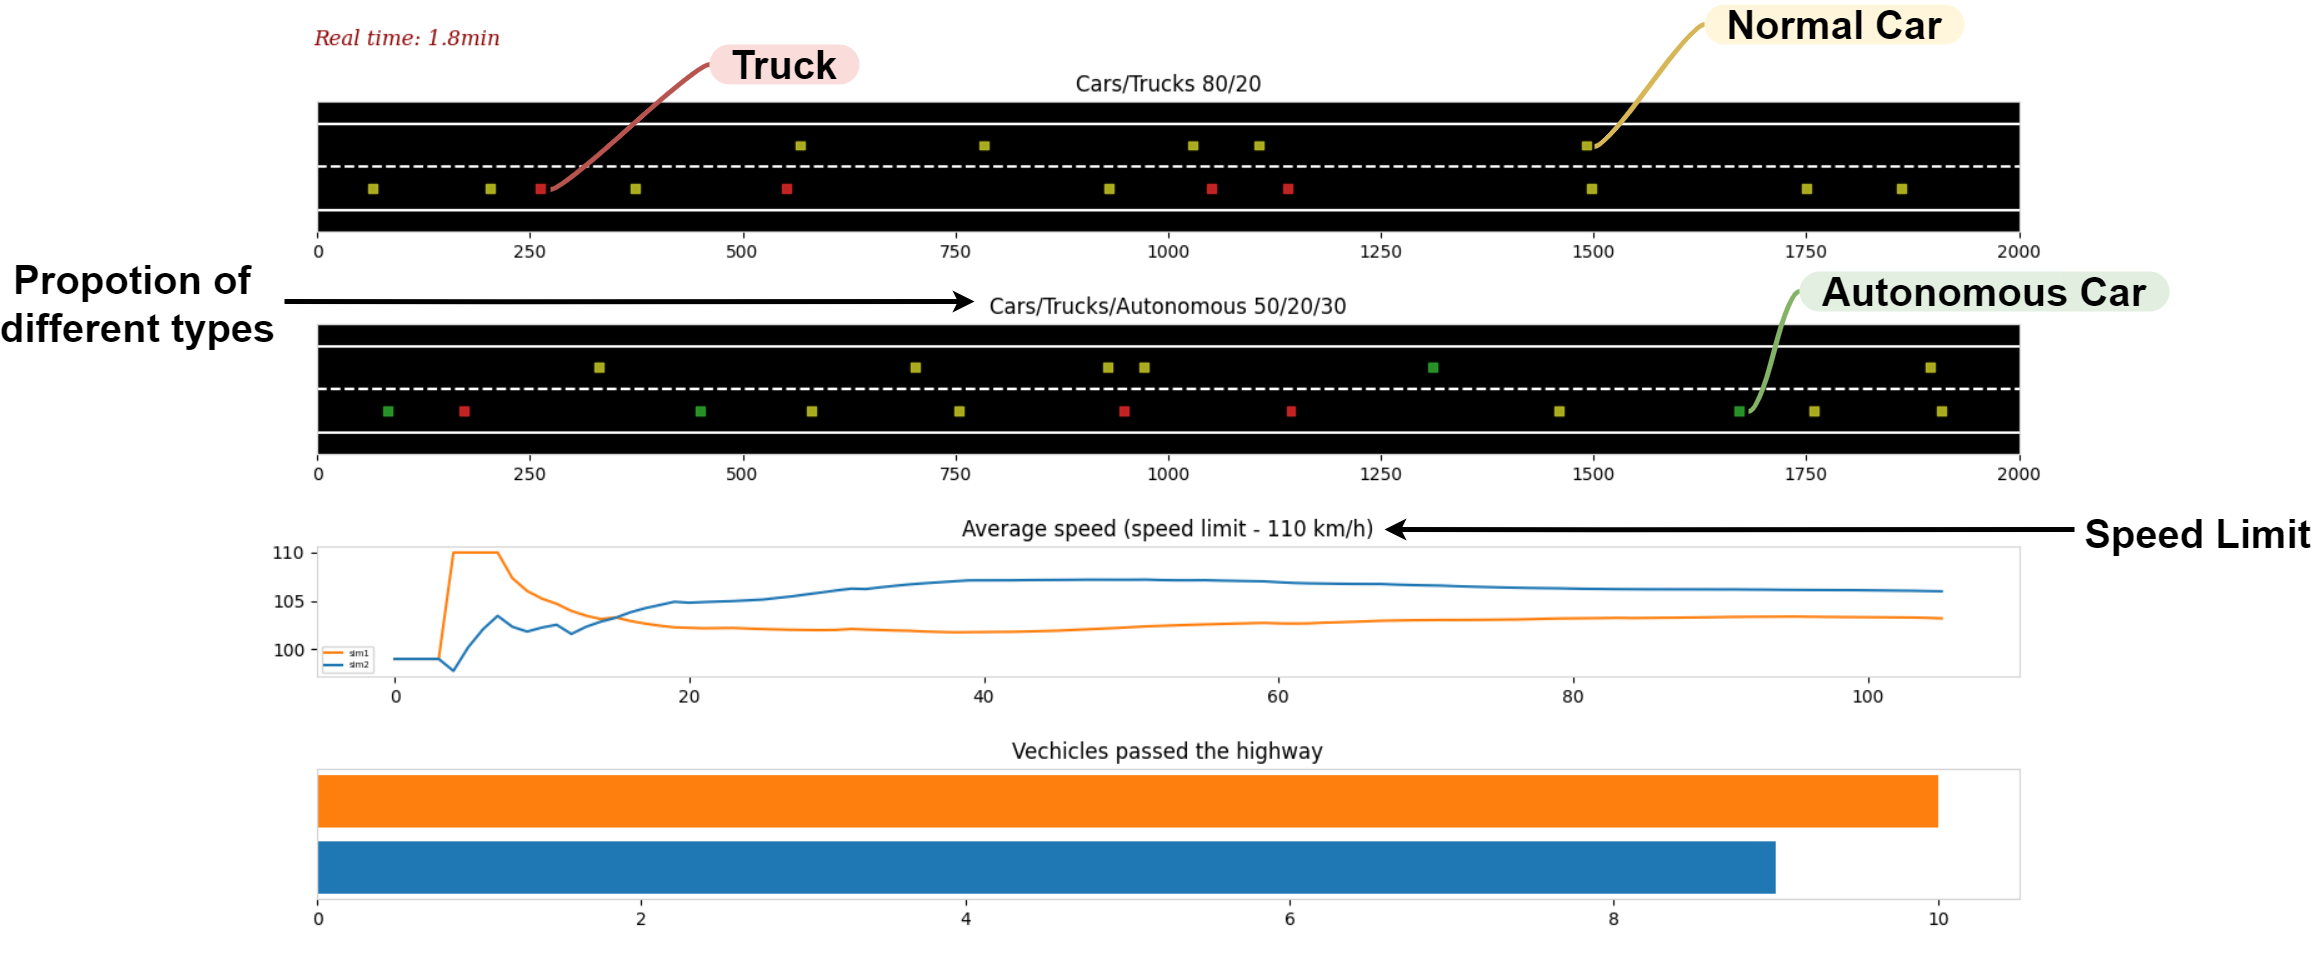
\includegraphics[width=\linewidth]{images/sim-colors-annotate.png}
    \caption{Coloring of different types of vehicles.}
    \label{fig:color-output}
\end{figure}

\section{JSON schema}
\label{appendix:json-schema}
\begin{figure}[H]
    \centering
    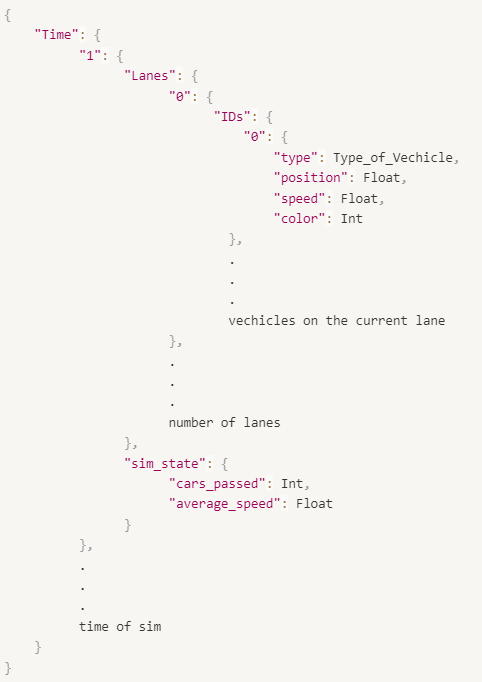
\includegraphics[width=0.5\linewidth]{images/json-schema.png}
    \caption{JSON schema}
    \label{fig:json-schema}
\end{figure}